\scanpage{103}

\[
\begin{array}{ccc@{\qquad}l}
P\times&Q\mathrel{\unsure{-|\to}}&R&Q\simeq R\\
e&e&e&P\simeq R
\end{array}
\qquad
\]\[G\times G\longrightarrow G\]

\diagram{\begin{tikzcd}[ampersand replacement=\&,row sep=small,column sep=small]
 \&P\ \ x\\
 \&\unsure{\gamma|\sigma}\ \Gamma\mathrel{-}\arrow[u,"p"]\arrow[dr,"q"]\arrow[dl,"r"']\\
 R\&\&Q\ \ y\\
 z
\end{tikzcd}}

\[
p(\gamma)\qquad q(\gamma)\qquad r(\gamma)
\qquad\begin{matrix} Q\\\unsure{\wr|21|\simeq}\\R\end{matrix}
\]

\[
\begin{aligned}
\left\{\begin{aligned}
y&\underset{p(\gamma)}{\sim}z\\
z&\underset{q(\gamma)}{\rightsquigarrow}x
\end{aligned}\right.
&\qquad\begin{aligned}
\Longleftrightarrow\exists(p(\gamma),y,z)&\in\Gamma\\
(x,q(\gamma),z)&\in\Gamma
\end{aligned}\\
?\ \Downarrow&\\
x\underset{r(\gamma)}{\sim}y&\qquad (x,y,r(\gamma))\in\Gamma
\end{aligned}
\]

\diagram{\begin{tikzcd}[ampersand replacement=\&,row sep=small,column sep=small]
 \&\widetilde P_u/\unsure{\sigma|G}\\
 \&\widetilde\Gamma/\sigma\arrow[u]\arrow[dl]\arrow[dr]\\
 \widetilde P_w/\sigma\&\&\widetilde P_v/\sigma
\end{tikzcd}}

\diagram{%
\begin{tikzcd}[ampersand replacement=\&,column sep=0pt,row sep=0pt]
|[inner sep=0pt]| \vcenter{\hbox{%
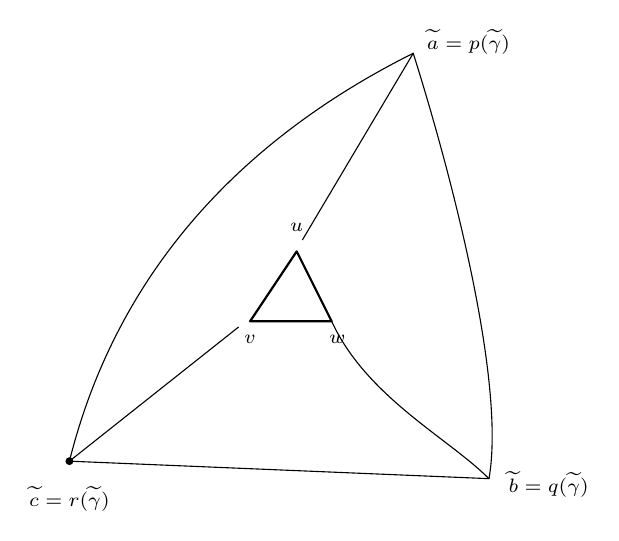
\begin{tikzpicture}[x=0.074cm,y=-0.074cm,line cap=round,line join=round,line width=.4pt]
\draw (59,0) .. controls (29,15) and (8,38) .. (0,70);
\draw (0,70) -- (72,73);
\draw (72,73) .. controls (75,56) and (65,19) .. (59,0);
\draw[thick] (39,34) -- (31,46) -- (45,46) -- cycle;
\draw (59,0) -- (40,32);
\draw (0,70) -- (29,47);
\draw (45,46) .. controls (51,59) and (65,66) .. (72,73);
\fill (0,70) circle[radius=0.05cm];
\node[inner sep=.55pt,anchor=west,font=\scriptsize] at (61,-2) {$\widetilde a=p(\widetilde\gamma)$};
\node[inner sep=.55pt,anchor=west,font=\scriptsize] at (75,74) {$\widetilde b=q(\widetilde\gamma)$};
\node[inner sep=.55pt,anchor=north,font=\scriptsize] at (0,74) {$\widetilde c=r(\widetilde\gamma)$};
\node[inner sep=.55pt,anchor=south,font=\scriptsize] at (39,31) {$u$};
\node[inner sep=.55pt,anchor=north,font=\scriptsize] at (31,48) {$v$};
\node[inner sep=.55pt,anchor=north,font=\scriptsize] at (46,48) {$w$};
\end{tikzpicture}%
}}
\end{tikzcd}%
}

\[\begin{aligned}ayz^{-1}&=1\\x^{-1}bz&=1\\xy^{-1}&\ \unsure{=1}\end{aligned}\]

\[
(a,b,c)\qquad abc=1\quad c=b^{-1}a^{\unsure{-|-1}}
\]
\[
abc=1\qquad
\left.\begin{aligned}ayz&=1\\xbz&=1\end{aligned}\right\}\ \overset{?}{\Downarrow}
\quad xyc=1\qquad\text{i.e.}
\]

\[
\begin{aligned}
ay&=xb\qquad y=a^{-1}xb\\xy&=xa^{-1}xb\\bca&=1\\x^{-1}ayca&=1
\end{aligned}
\]

\[
\begin{aligned}
&\deleted{xyz=}\qquad z=(ay)^{-1}\\
&x=(bz)^{-1}=z^{-1}b^{-1}=ayb^{-1}\deleted{=ayca}\\
&?\Downarrow\quad y=x^{-1}c^{-1}=by^{-1}a^{-1}c^{-1}
=\deleted{\unsure{by^{-1}b|byc^{-1}b}}\ b\deleted{\unsure{(cay)^{-1}}}\\
&\qquad\deleted{\unsure{x=cy(yaby^{-1})}}\\
&\qquad=by^{-1}b^{\unsure{a|1|-1}}=\operatorname{int}(b)y^{-1}
\end{aligned}
\]

\[
\begin{aligned}
&b\,(by^{-1}b^{-1}\qquad\qquad \deleted{c^{-1}y^{-1}}\qquad aby^{-1}=ayb^{-1}\\
&\operatorname{int}(b)\bigl(\operatorname{int}(b)y^{-1}\bigr)^{-1}
\qquad b(by^{-1}b)^{-1}b\\
&\operatorname{int}(b)\,(\operatorname{int}(b)(y))\qquad
b\,b^{-1}yb^{-1}b\qquad by^{-1}=yb^{-1}\qquad (by^{-1})^2=\underline{1}
\end{aligned}
\]

% archive sheet number: 104
